\Titre{Extended Berkeley Packet Filter}
\usepackage{ifthen}


\def\txthl#1{ \ifthenelse{\lengthtest{#1 pt<0.5pt}}{\top}{\bot} }



\makeatletter
\def\verbatim@font{\tiny\ttfamily}
\makeatother
\begin{document}

\begin{reveals}
                
\maketitle

\section{Context}

\begin{frame}[c,fragile]{Programs}
  
  \begin{block}{Program file}
    \begin{itemize}
    \item An \emph{object} file contains the instructions, as well as
      functions' and static data addresses
    \item All addresses are stored in a \emph{symbol table}
    \item Undefined functions have to be found by the system at execution time
      \begin{center}
        \color{red}Dynamic libraries \textit{vs} Static libraries
      \end{center}
    \item \texttt{objdump -T prog} shows the symbol table of a program 
    \end{itemize}
  \end{block}

\begin{verbatim}
0000000000000000      DF *UND*	0000000000000000  GLIBC_2.2.5 freeaddrinfo
0000000000000000      DF *UND*	0000000000000000  GLIBC_2.3.4 __sprintf_chk
0000000000000000      DF *UND*	0000000000000000  GLIBC_2.2.5 socket
000000000048eb80 g    DF .text	00000000000000b3  Base        camlBiblio__cut_after_nth_rec_1221
00000000004702f0 g    DF .text	0000000000000059  Base        camlConstraints__fun_1645
000000000047a610 g    DF .text	000000000000002f  Base        camlUnif_AC__fun_3543
000000000049fac0 g    DF .text	0000000000000122  Base        camlHashtbl__remove_1185
00000000006d77a0 g    D  .data	0000000000000000  Base        caml_exn_Stack_overflow
\end{verbatim}

\end{frame}

\begin{frame}[c,fragile]{Process Execution}
  
  \begin{block}{Operating system's job}
    \begin{enumerate}[<-+>]
    \item Load a program file in memory
    \item Provide virtual addresses as well as real addresses (in memory)
    \item Map virtual addresses to real addresses
      \begin{center}
        \color{red}Partial mapping, hence Segfaut
      \end{center}
    \item (Optionally) add a random offset for the base addresses of functions
    \item Start execution at address 0 of the text
    \item Initialisation is provided by the RunTime library
      (\textit{e.g.} libcrt), which calls \texttt{main}
    \end{enumerate}
  \end{block}
  
\end{frame}

\begin{frame}[c,fragile]{Program Modification}
  
  \begin{block}{Kernel-side}
    \begin{enumerate}[<-+>]
    \item The OS can replace calls to functions by other calls
    \item The OS can insert and delete in memory instructions at any place
    \end{enumerate}
  \end{block}
  \vfill
  \begin{block}{User-side}
    \begin{enumerate}[<-+>]
    \item Needs to be root, have the \texttt{SYS\_PTRACE} capability
      (Linux), or own the process
      \begin{center}
        *BSD: for non-root users, must be the parent of the process
      \end{center}
    \item The \emph{ptrace} call allows for the reading and writing at
      runtime of a process memory (and of the registers)
    \end{enumerate}
  \end{block}
  
\end{frame}

\begin{frame}[c]{eBPF}
  
  \begin{block}{The language}
    \begin{itemize}
    \item Bytecode language
    \item Can be interpreted (like Java) by a Virtual Machine
    \item Can be compiled at run time (like JavaScript) into Machine Code 
    \end{itemize}
  \end{block}


  \begin{block}{Kernel Support}
    \begin{itemize}
    \item An eBPF JIT compiler
    \item A \emph{sandbox} (with restricted memory access for spatial
      separation) for the execution of the compiled code
    \item A \emph{verifier} that verifies the time separation of the code
    \item A module that receives commands from Userland to perform
      runtime modification
      \begin{itemize}
      \item On users' code (uprobe)
      \item On kernel's code (kprobe)
      \end{itemize}
    \item Communication: shared memory or file
    \end{itemize}
  \end{block}


\end{frame}



\section{BPFTrace}

\subsection{BPFTrace snippet}

\definecolor{deepblue}{RGB}{0,0,64}

\begin{frame}[c]{Presentation}
  \framesubtitle{From \emph{BPFTrace Internals}, Jiri Olsa, 2020} 
  
  \begin{center}
    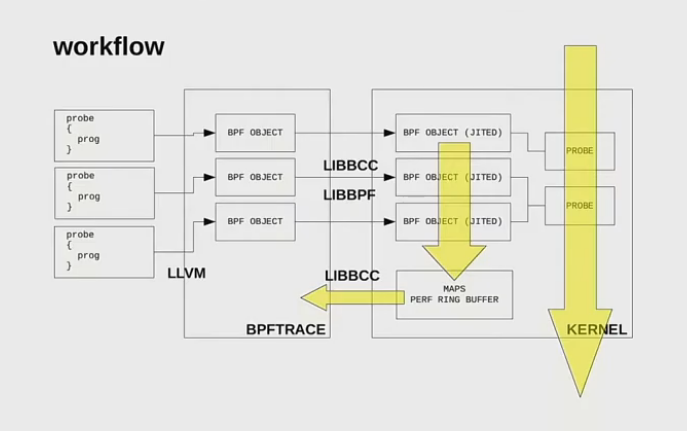
\includegraphics[width=0.8\textwidth]{images/BPFTrace-workflow.png}
  \end{center}

\end{frame}

\begin{frame}[c]{The eBPF Bytecode}
  
  \begin{center}
      \color{deepblue}
    \begin{tabular}{|ll|}
      \arrayrulecolor{deepblue}
      \multicolumn 2{|l|}{\cellcolor{deepblue}\textcolor{white}{Environment}}\\
      r<1-10>& registers \\
      r<1-5> & func arguments\\
      r0 & return value\\
      r10 & stack on entry \\
      r1 & context on entry\\
      map[id:X] & map descriptor\\\hline
    \end{tabular}
  \end{center}

  \vfill

  \begin{block}{Remarks}
    \begin{itemize}
    \item Maps are associative tables
    \item Maps are the effective way to store information
    \item Possible calls to helper functions 
    \item Very limited stack size (512b)
    \end{itemize}
  \end{block}

\end{frame}

\begin{frame}[c,fragile]{Using maps (1/2)}
  \framesubtitle{Using a C interface}
  
  \begin{block}{Map update}
\begin{lstlisting}[language=C]
int (*bpf_map_update_elem ) ( 
            void * map ,
            const void * key ,
            const void * value ,
            uint64_t flags ) ;
\end{lstlisting}
  \end{block}

  \vfill

  \begin{block}{Remarks}
    \begin{itemize}
    \item Most maps are hashtables (\textit{i.e.}
      \lstinline[language=C]|_htab_map_update_elem| or
      \lstinline[language=C]|_htab_percpu_map_update_elem|)
    \item Translation is provided for the supported languages!
    \item Map Ids (the pointer map) are shared between calls 
    \end{itemize}
  \end{block}

\end{frame}

\begin{frame}[c,fragile]{Using maps (2/2)}
  \framesubtitle{Using a C interface}
  
  \begin{block}{Map lookup}
\begin{lstlisting}[language=C]
const void * 
(*bpf_map_lookup_elem ) ( 
            void * map ,
            const void * key ) ;
    \end{lstlisting}
  \end{block}

  \vfill

  \begin{block}{Remarks}
    \begin{itemize}
    \item returns NULL if the key is not in the map
    \item returns the stored value (of type \lstinline[language=C]|const void *|)
    \end{itemize}
  \end{block}

\end{frame}

\begin{frame}[c]{Maps from BPFTrace}
  
  \begin{center}
      \color{deepblue}
    \begin{tabular}{|ll|}
      \arrayrulecolor{deepblue}
      \multicolumn 2{|l|}{\cellcolor{deepblue}\textcolor{white}{BPFTrace}}\\
      @, @[name(,name)*] & default map, map \emph{name} \\
      count(\emph{name}) & number of elements\\\hline
    \end{tabular}
  \end{center}

\end{frame}

\begin{frame}[c,fragile]{Variables}

  \begin{block}{Naming}
\begin{lstlisting}[language=C]
@name = 0;      
\end{lstlisting}
  \end{block}

  \vfill

  \begin{center}
      \color{deepblue}
    \begin{tabular}{|p{0.4\textwidth}p{0.4\textwidth}|}
      \arrayrulecolor{deepblue}
      \multicolumn 2{|l|}{\cellcolor{deepblue}\textcolor{white}{Variables use}}\\
      @\emph{name} & Global variable \emph{name} of type int \\
      \$\emph{name} & Per-event variable \emph{name} of type int \\
      toto, gcc & string constants/names\\
      arithmetics & as in C\\
      printf & as in C\\
      min, max, avg, sum, stats, hist, lhist & aggregates on all calls using internally a map\\\hline
    \end{tabular}
  \end{center}

\end{frame}

\begin{frame}[c,fragile]{Pre-defined Variables (1/2)}

      \begin{center}
        \color{deepblue}
        \begin{tabular}{|p{0.25\textwidth}p{0.6\textwidth}|}
          \arrayrulecolor{deepblue}
          {\cellcolor{deepblue}\textcolor{white}{Variable Name}} &
                                                          {\cellcolor{deepblue}\textcolor{white}{Meaning}} \\
pid & Process ID (kernel tgid)\\
tid & Thread ID (kernel pid)\\
uid & User ID\\
gid & Group ID\\
nsecs & Nanosecond timestamp\\
elapsed & Nanoseconds since bpftrace initialization\\
cpu & Processor ID\\
comm & Process name\\
kstack & Kernel stack trace\\
ustack & User stack trace\\\hline
        \end{tabular}
      \end{center}
\end{frame}
\begin{frame}[c,fragile]{Pre-defined Variables (2/2)}

      \begin{center}
        \color{deepblue}
        \begin{tabular}{|p{0.25\textwidth}p{0.6\textwidth}|}
          \arrayrulecolor{deepblue}
          {\cellcolor{deepblue}\textcolor{white}{Variable Name}} &
                                                          {\cellcolor{deepblue}\textcolor{white}{Meaning}} \\
          arg0,\(\ldots\), argN. & Arguments to the traced function; assumed to be 64 bits wide\\
sarg0, \(\ldots\), sargN. & Arguments to the traced function (for programs that store arguments on the stack); assumed to be 64 bits wide\\
retval & Return value from traced function\\
func & Name of the traced function\\
probe & Full name of the probe\\
curtask & Current task struct as a u64\\
rand & Random number as a u32\\
cgroup & Cgroup ID of the current process\\
cpid & Child pid(u32), only valid with the -c command flag\\
\$1, \$2, \ldots, \$N, \$\#. & Positional parameters for the bpftrace program\\\hline
        \end{tabular}
      \end{center}
\end{frame}

\begin{frame}[c]{Output}
  
  \begin{center}
      \color{deepblue}
    \begin{tabular}{|ll|}
      \arrayrulecolor{deepblue}
          {\cellcolor{deepblue}\textcolor{white}{Function Name}} &
                                                          {\cellcolor{deepblue}\textcolor{white}{Usage}} \\
      printf & prints at each event\\
      print(\emph{name}) & prints the map\\
      hist(\emph{name})& histogram (power of two)\\
      lhist(\emph{name},\emph{min},\emph{max},\emph{step})& histogram (linear)\\\hline
    \end{tabular}
  \end{center}
\end{frame}


\begin{frame}[c]{Calling external programms}
  
  \begin{block}{Built-in function \textcolor{red}{system}}
    \begin{itemize}
    \item Argument: printf-like format string
    \item Evaluates the string as a program to call 
    \item Needs an extra \texttt{--unsafe} flag
    \end{itemize}
  \end{block}

\end{frame}

\subsection{BPFTrace probes}

\begin{frame}[c]{Probe}
  
  \begin{block}{Definition}
    \begin{itemize}
    \item Location in a program where additional code has to be
      executed
    \item Can be either in the kernel or a position in the code of the
      program
    \end{itemize}
  \end{block}

  \vfill

  \begin{center}
      \color{deepblue}
    \begin{tabular}{|ll|}
      \arrayrulecolor{deepblue}
          {\cellcolor{deepblue}\textcolor{white}{Probe type}} &
                                                          {\cellcolor{deepblue}\textcolor{white}{Usage}} \\
      kprobe/kretprobe & Kernel function tracing\\
      uprobe/uretprobe& Programs function tracing\\
      tracepoint & Essentially system calls tracing\\
      usdt & Tracing of statically defined tracepoints\\
      interval & Time events (auxiliary)\\
      software & Kernel software events\\
      hardware & HW  events (cache miss, etc.)\\\hline
    \end{tabular}
  \end{center}


\end{frame}
Hardware events:

    cpu-cycles or cycles
    instructions
    cache-references
    cache-misses
    branch-instructions or branches
    branch-misses
    bus-cycles
    frontend-stalls
    backend-stalls
    ref-cycles


\begin{frame}[c,fragile]{Hardware events}
  
  \begin{center}
      \color{deepblue}
    \begin{tabular}{|p{.55\textwidth}p{.35\textwidth}|}
      \arrayrulecolor{deepblue}
          {\cellcolor{deepblue}\textcolor{white}{Name}} &
                                                          {\cellcolor{deepblue}\textcolor{white}{Raised when}} \\
          cpu-cycles or cycles& \\
    instructions& \\
    cache-references& \\
    cache-misses& \\
    branch-instructions or branches& \\
    branch-misses& \\
    bus-cycles& \\
    frontend-stalls& \\
    backend-stalls& \\
    ref-cycles& \\\hline
    \end{tabular}
  \end{center}

\end{frame}



\begin{frame}[c,fragile]{Software Events}
  \begin{center}
      \color{deepblue}
    \begin{tabular}{|p{.55\textwidth}p{.35\textwidth}|}
      \arrayrulecolor{deepblue}
          {\cellcolor{deepblue}\textcolor{white}{Name}} &
                                                          {\cellcolor{deepblue}\textcolor{white}{Raised when}} \\
    cpu-clock or cpu& \\
    task-clock& \\
    page-faults or faults& \\
    context-switches or cs& \\
    cpu-migrations& \\
    minor-faults& \\
    major-faults& \\
    alignment-faults& \\
    emulation-faults& \\
    dummy& \\
    bpf-output& \\\hline
    \end{tabular}
  \end{center}
\end{frame}




% usdt:\emph{path}:\emph{name} & user defined static tracing, needs systemtap/dtrace for preparing the program\\
% \lstinline[language=awk]|usdt:/root/tick:loop { printf("%s: %d\n", str(arg0), arg1); }|
% \begin{frame}[c,fragile]{User defined}
%   \begin{center}
%       \color{deepblue}
%     \begin{tabular}{|p{.25\textwidth}p{.65\textwidth}|}
%       \arrayrulecolor{deepblue}
%           {\cellcolor{deepblue}\textcolor{white}{}} &
%                                                           {\cellcolor{deepblue}\textcolor{white}{}} \\
%     \end{tabular}
%   \end{center}
%\end{frame}


\begin{frame}[c,fragile]{Userland Probes}
  
  \begin{center}
      \color{deepblue}
    \begin{tabular}{|p{.60\textwidth}p{.30\textwidth}|}
      \arrayrulecolor{deepblue}
          {\cellcolor{deepblue}\textcolor{white}{Syntax}} &
                                                          {\cellcolor{deepblue}\textcolor{white}{Example}} \\
      uprobe:library\_name:function\_name[+offset] & path to a library and relative address from a function start\\
      uprobe:library\_name:address & path to a library and absolute address in text\\
      uprobe:path:function\_name[+offset] & path to an object file and relative address from a function start\\
      uprobe:path:address & path to an object file and absolute address in text\\\hline
    \end{tabular}
  \end{center}
  \vfill
  \begin{center}
      \color{deepblue}
    \begin{tabular}{|ll|}
      \arrayrulecolor{deepblue}
          {\cellcolor{deepblue}\textcolor{white}{Call}} &
                                                          {\cellcolor{deepblue}\textcolor{white}{Automatic variables}} \\
      uprobe&  arguments arg0, arg1, \ldots, argN\\
      uretprobe&  return value in retval\\\hline
    \end{tabular}
  \end{center}
\end{frame}

\begin{frame}[c,fragile]{Userland Probes}
  
  \begin{center}
      \color{deepblue}
    \begin{tabular}{|p{.60\textwidth}p{.30\textwidth}|}
      \arrayrulecolor{deepblue}
          {\cellcolor{deepblue}\textcolor{white}{Syntax}} &
                                                          {\cellcolor{deepblue}\textcolor{white}{Example}} \\
      uprobe:library\_name:function\_name[+offset] & path to a library and relative address from a function start\\
      uprobe:library\_name:address & path to a library and absolute address in text\\
      uprobe:path:function\_name[+offset] & path to an object file and relative address from a function start\\
      uprobe:path:address & path to an object file and absolute address in text\\\hline
    \end{tabular}
  \end{center}
  \vfill
  \begin{block}{Examples}
    One can get the files opened or the user input in terminals with:
\begin{lstlisting}[language=Awk]
uprobe:/lib/x86_64-linux-gnu/libc-2.31.so:fopen { \
                  printf("file opened: \"%s\"\n", str(arg0)); }
uretprobe:/bin/bash:readline { \
                  printf("readline: \"%s\"\n", str(retval)); }
\end{lstlisting}
  \end{block}
\end{frame}


\begin{frame}[c,fragile]{Kernel Probes}
  
  \begin{center}
      \color{deepblue}
    \begin{tabular}{|p{.5\textwidth}p{.4\textwidth}|}
      \arrayrulecolor{deepblue}
          {\cellcolor{deepblue}\textcolor{white}{Syntax}} &
                                                          {\cellcolor{deepblue}\textcolor{white}{Example}} \\
      kprobe:function\_name[+offset] & Kernel function when called, with relative address \\
      kretprobe:function\_name & Kernel function return value\\\hline
    \end{tabular}
  \end{center}
  \vfill
  \begin{center}
      \color{deepblue}
    \begin{tabular}{|ll|}
      \arrayrulecolor{deepblue}
          {\cellcolor{deepblue}\textcolor{white}{Call}} &
                                                          {\cellcolor{deepblue}\textcolor{white}{Automatic variables}} \\
      kprobe&  arguments arg0, arg1, \ldots, argN\\
      kretprobe&  return value in retval\\\hline
    \end{tabular}
  \end{center}
\end{frame}
\begin{frame}[c,fragile]{Kernel Probes}
  
  \begin{center}
      \color{deepblue}
    \begin{tabular}{|p{.5\textwidth}p{.4\textwidth}|}
      \arrayrulecolor{deepblue}
          {\cellcolor{deepblue}\textcolor{white}{Syntax}} &
                                                          {\cellcolor{deepblue}\textcolor{white}{Example}} \\
      kprobe:function\_name[+offset] & Kernel function when called, with relative address \\
      kretprobe:function\_name & Kernel function return value\\\hline
    \end{tabular}
  \end{center}
  \vfill
  \begin{block}{Examples}
    One can get all the files opened on the system with:
\begin{lstlisting}[language=Awk]
kprobe:do_sys_open { printf("opening: %s\n", str(arg1)); }'
\end{lstlisting}
  \end{block}
\end{frame}



\begin{frame}[c,fragile]{Tracepoints}
  \framesubtitle{Mostly for system calls}

  \begin{center}
      \color{deepblue}
    \begin{tabular}{|p{.6\textwidth}p{.3\textwidth}|}
      \arrayrulecolor{deepblue}
          {\cellcolor{deepblue}\textcolor{white}{Syntax}} &
                                                          {\cellcolor{deepblue}\textcolor{white}{Called when}} \\
      tracepoint:syscalls:sys\_enter\_\emph{name} &
                                                                            When a program makes the \emph{name} system call\\
      tracepoint:syscalls:sys\_exit\_\emph{name} &
                                                                            When the system call \emph{name} returns \\\hline
    \end{tabular}
  \end{center}
  \vfill
  \begin{center}
      \color{deepblue}
    \begin{tabular}{|p{.25\textwidth}p{.65\textwidth}|}
      \arrayrulecolor{deepblue}
          {\cellcolor{deepblue}\textcolor{white}{Type}} &
                                                          {\cellcolor{deepblue}\textcolor{white}{Called when}} \\
      enter & pid making the call, and the arguments\\
      exit & pid to which the value is returned, and the returned value (dependent on each system call)\\\hline
    \end{tabular}
  \end{center}

  \vfill

  \begin{block}{Which values are available?}
\begin{lstlisting}[language=bash]
cat /sys/kernel/debug/tracing/events/syscalls/\
      sys_enter_open/format
\end{lstlisting}
\begin{verbatim}
name: sys_enter_openat
ID: 608
format:
	field:unsigned short common_type;	offset:0;	size:2;	signed:0;
	field:unsigned char common_flags;	offset:2;	size:1;	signed:0;
...
\end{verbatim}

  \end{block}

\end{frame}


\begin{frame}[c,fragile]{Time Events (Interval)}
  
  \begin{block}{Goal}
    \begin{itemize}
    \item ``Synthetic'' event to perform something periodically
    \item syntax: \texttt{interval:time}
    \item time is in microseconds (us), milliseconds (ms), seconds
      (s), or every \(n\) per second (Hz)
    \item Normally used with another probe, and with the two probes
      sharing (at least) a global variable
    \end{itemize}
  \end{block}

\end{frame}


\subsection{BPFTrace programs}



\begin{frame}[c,fragile]{BPFTrace Programs}
  
  \begin{block}{Structure}
    \begin{itemize}
    \item A BPFTrace programm attaches code snippets with conditions
      to probes (see examples above)
      \begin{center}
        Conditionals can use the automatic variables, are in / \ldots /
        between the probe and the code
      \end{center}
    \item Two additional probes:
      \begin{description}
      \item[BEGIN:] to initialise maps and data, code executed before
        all other code
      \item[END:] code executed when exiting the program, useful for
        printing stats
      \end{description}
    \end{itemize}
  \end{block}

  \vfill

  \begin{center}
    Same as Awk programs!
  \end{center}


  \begin{block}{Calling BPFTrace}
\begin{lstlisting}[language=bash]
 bpftrace -e 'kprobe:do_nanosleep \
          /tid == 1234/ { printf("sleep by %d\n", tid); }'   
\end{lstlisting}
  \end{block}



\end{frame}


\section{Conclusion}

\begin{frame}[c]{To delve further\(\ldots\)}
  
  \begin{block}{G\raisebox{0.6ex}{al} K. Alexander}
    The difference between you and us is that we \textcolor{red}{know} what runs on a system
  \end{block}

  

  \begin{description}
  \item[man bpf-helpers:] not always current list of functions
  \item[kernel code:] headers or src
    \begin{itemize}
    \item \url{include/uapi/linux/bpf.h}: all heper functions
    \item \url{net/core/filter.c}: network related functions
    \item \url{kernel/trace/bpf_trace.c}: tracing functions
    \item \url{kernel/bpf/}: other functions (cgroups,...)
    \end{itemize}
  \item[bpftool:] \lstinline[language=bash]|bpftool feature probe|
    gives the name of existing functionalities in the running kernel
  \end{description}
\end{frame}


\begin{frame}[c]{To delve further\(\ldots\)}
  
  \begin{block}{G\raisebox{0.6ex}{al} K. Alexander}
    The difference between you and us is that we \textcolor{red}{know} what runs on a system
  \end{block}


\end{frame}
\end{reveals}

\end{document}


